\chapter{Heap and Sequential Organizations}

\section{Storing Collections of Records}
\begin{itemize}
    \item A database is primarily made of \textbf{tables of records}, each one implemented by the \textit{Storage Structures Manager} as a \textbf{file of pages} provided by the \textit{Permanent Memory Manager}
    \item Pages are assumed to be of a fixed size and to contain several records
    \item The \textbf{unit of cost} for data access is a \textit{page access}
    \item The most important \textit{type of file} is the \textbf{heap file}, which stores records in no particular order, and provides a record at a time interface for accessing, inserting and deleting records
\end{itemize}

\subsection{Record Structure}
\begin{itemize}
    \item Each record consists of one or more \textit{attributes} and contains several additional bytes, called \textit{record header} useful for record management
    \item \textit{Record header} generally contain:
    \begin{itemize}
        \item Information on the length of the record
        \item The number of attributes
        \item Whether the record has been deleted
        \item The name of the file to which it belongs
    \end{itemize}
\end{itemize}
We will assume that records are not larger than a page and that the values of the attributes are stored according to one of the strategies shown:
\begin{figure}[!h]
        \centering
        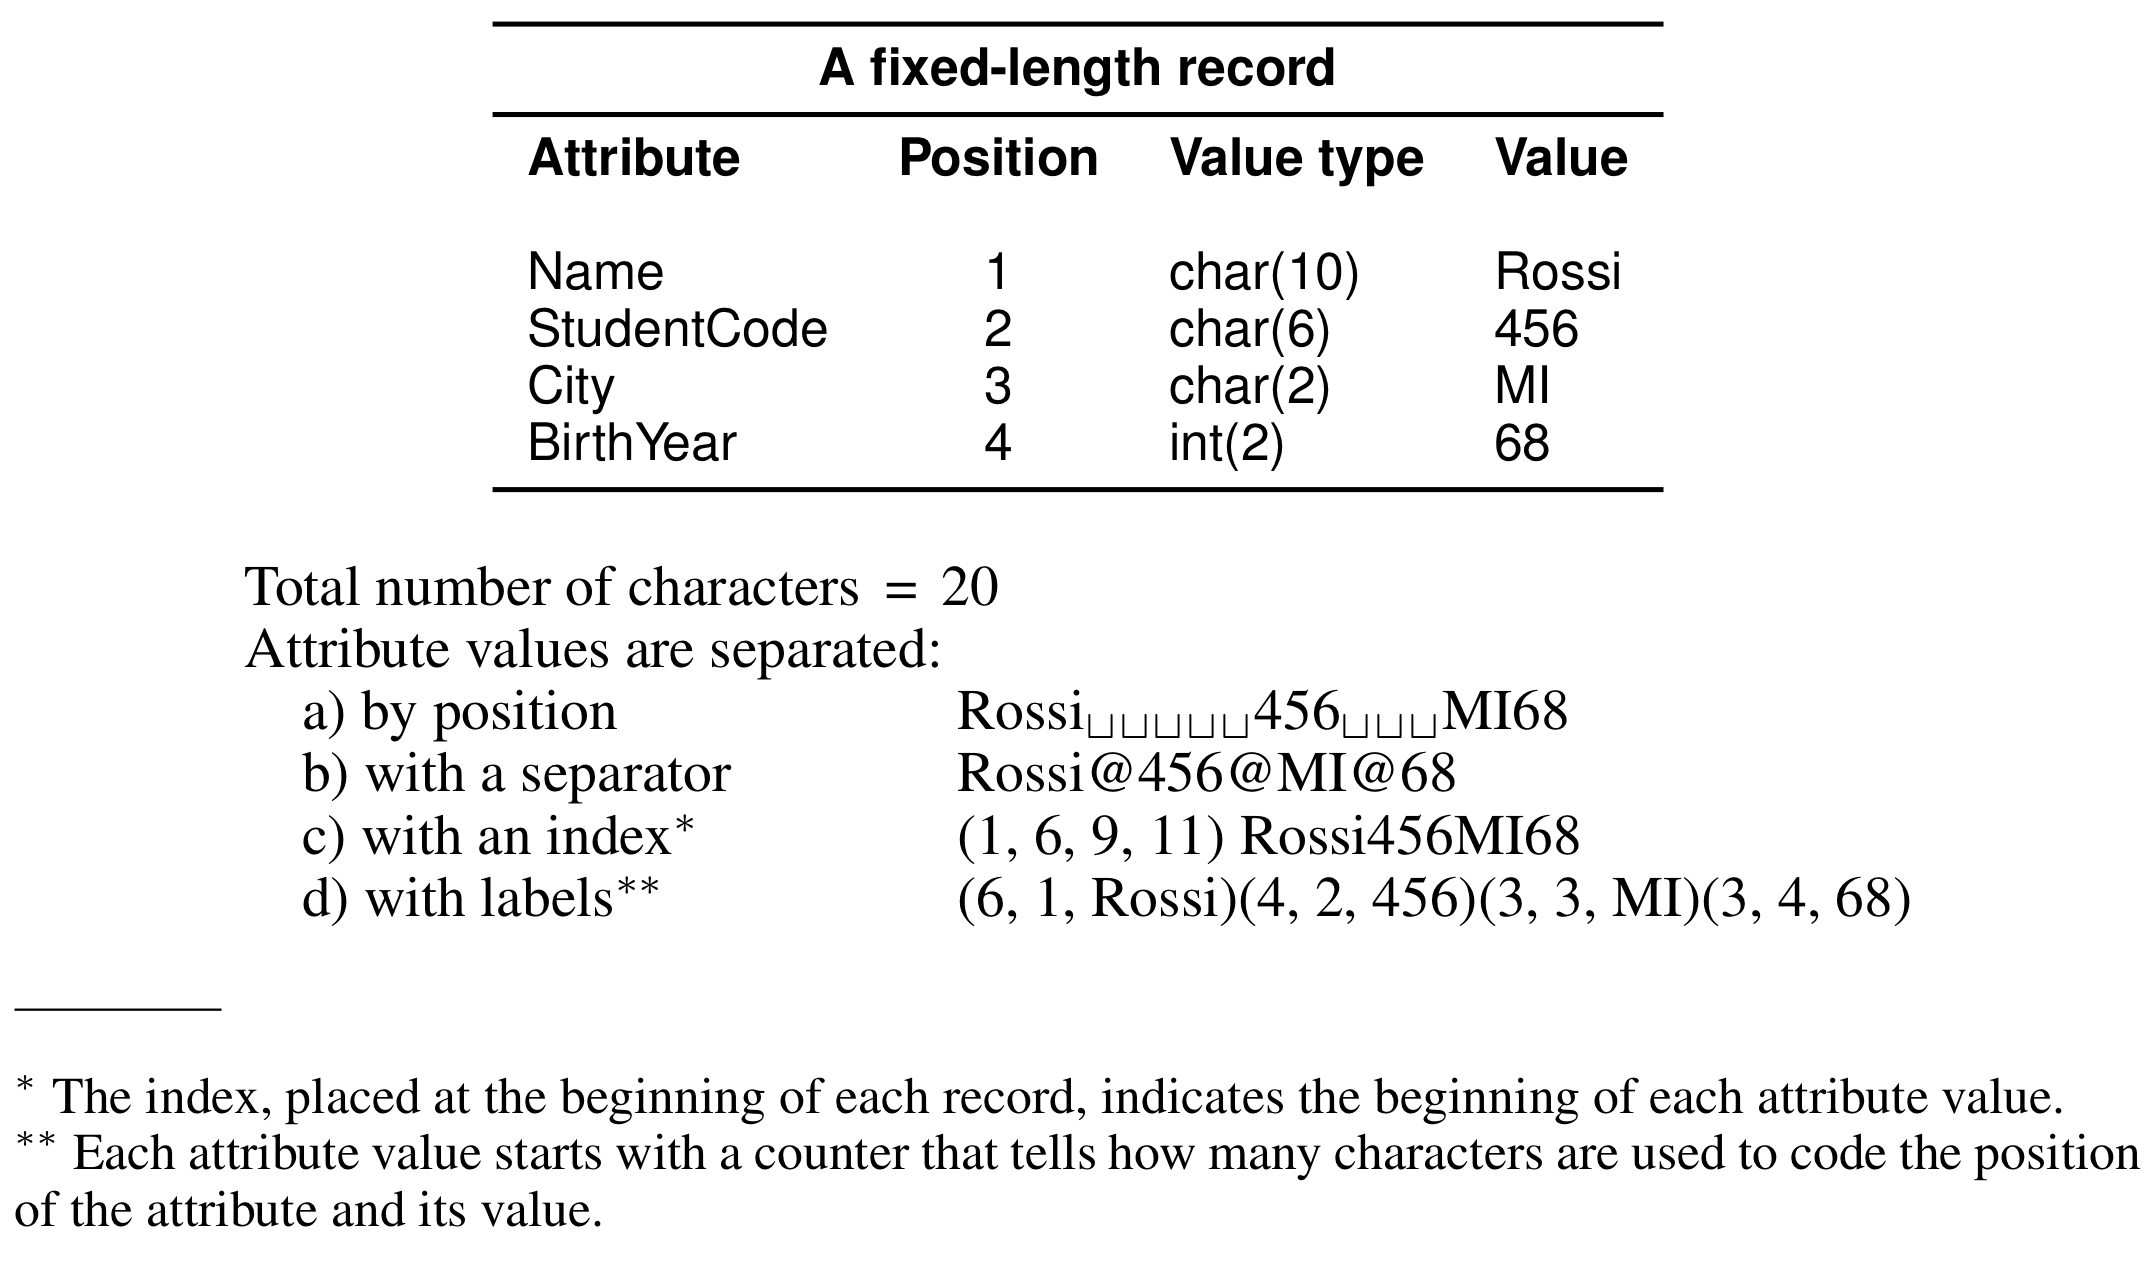
\includegraphics[width=0.7\linewidth]{images/DBMS_Internals/attribute_values.jpeg}
        \caption{Representation of attribute values}
    \end{figure}

\newpage
\subsection{Page Structure}
\begin{itemize}
    \item When a record is stored in the database, it is identified by a \textbf{record identifier} or \textbf{tuple identifier (RID)}, used like a pointer to record
\end{itemize}
\begin{figure}[!h]
        \centering
        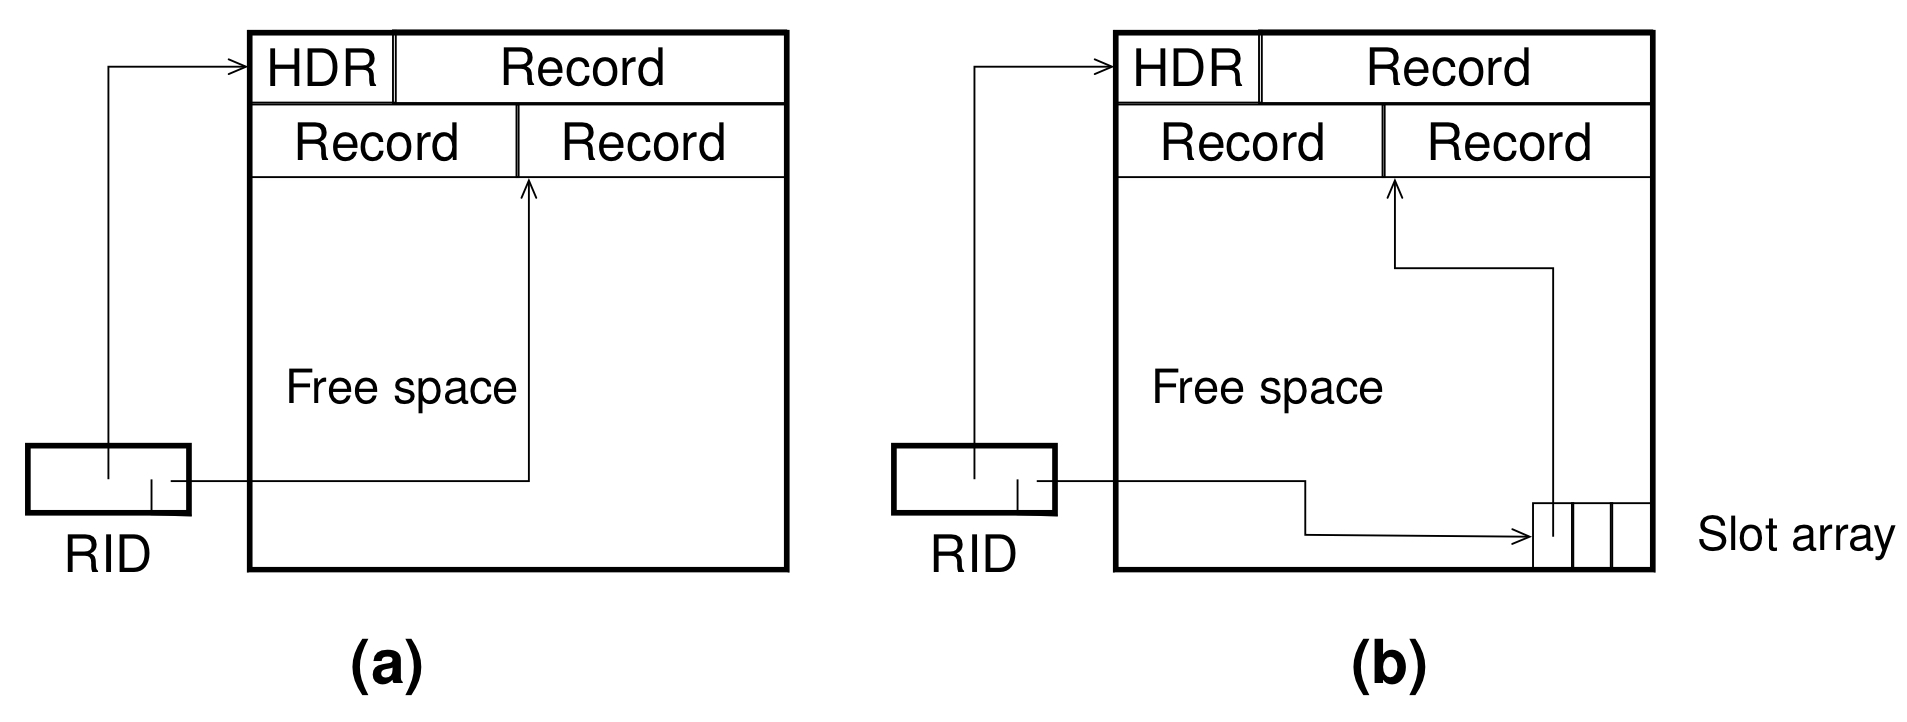
\includegraphics[width=0.7\linewidth]{images/DBMS_Internals/pointers_to_records.jpeg}
        \caption{Pointers to records}
\end{figure}
The exact nature of a RID can vary from one system to another:
\begin{itemize}
    \item We could take its \textbf{address (a)}. But this solution is not satisfactory because a record that contains variable-length attributes of type \textit{varchar} are themselves variable-length strings within a page
    \item RID formed by \textbf{two parts (b)} \textit{(Page number, Slot number)}. Where the slot number is an index into an array stored at the end of the page, called \textbf{slot array}.
\end{itemize}
If an updated record moves within its page, the local address in the array only must change, while the RID does not change. If an updated record cannot be stored in the same page because of lack of space, then it will be stored in another page, and the original record will be replaced by a forwarding pointer.

Each page has a \textbf{page header} that contains administrative information like:
\begin{itemize}
    \item The number of free bytes in the page
    \item The reference at the beginning of the free space
    \item The reference to the next not empty page of the file
\end{itemize}

\subsection{File Pages Management}
When a record is inserted into a collection, assuming that the records have size smaller than a page, the file manager proceeds as follows:
\begin{itemize}
    \item A file page is selected that contains free space for the new record; if the page does not exist, the file is extended with a new page. Let Let \(P\) be the address of the page where the record will be stored
    \item A reference to the beginning of the record is stored in the first free location \(j\) of the directory of slots of the page \(P\)
    \item The RID\((P, j)\) is assigned to the record
\end{itemize}

To implement insertion, the system uses a \textit{table} stored on disk, containing pairs of \textit{(fileName, headerPage)}, where the header page is the first page of the file, and the following alternatives are usually considered:
\begin{itemize}
    \item The heap file pages are organized as \textit{two double linked list} of pages, those full and those with free space
    \item In the header is stored a directory of pages and each entry contains the pair (page identifier, the amount of free space on the page). If the directory grows and cannot be stored in the header page, it is organized as a linked list. The information about the amount of free space on a page is used to select a page with enough space to store a record to be inserted
\end{itemize}
Finally, for reasons of efficiency, the free space existing in different pages is not compacted in one page by moving records. Therefore, it may happen that, due to a lack of available pages, it is not possible to assign a new free page despite the fact that the overall free space in different pages is greater than the total capacity of a page.

\newpage
\section{Cost Model}
The most important criteria to evaluate a file organization are the \textbf{amount of memory occupied} and the \textbf{cost of the basic operations}.
\begin{tcolorbox}
The most important operation is the search, because the first step for all operations is to check whether a record exists.
\end{tcolorbox}
We will estimate the value of the following parameters:
\begin{itemize}
    \item \(N_{rec}(R)\): number of record stored in file \(R\)
    \item \(L_r\): record length
    \item \(N_{pag}(R)\): number of pages where the record is stored
    \item \(D_{pag}\): page size
\end{itemize}
The operations cost will be estimated by considering only the operations to read and write a file page. The cost of the operations will be expressed in terms of the number of permanent memory accesses.

When, in some instances, we want to emphasize the magnitude of the execution time, we will make the simplifying assumption that the time to perform an operation is a simple function of the number of access operations:
\[ExecutionTime = NoAccesses \times OneAccessAverageTime\]

\section{Heap Organization}
\begin{tcolorbox}
The simplest way to organize data is to store it in file pages in the insertion order rather than sorted by a key value. The heap organization is the default solution used by DBMSs, and it is adequate for:
\begin{itemize}
    \item Small collection of records
    \item Infrequent key search 
\end{itemize}
\end{tcolorbox}

\subsection{Performance Evaluation - (NOT REQUIRED)}
\begin{itemize}
    \item \textbf{Memory Requirements:} the \textit{memory occupied} by a heap organization is only that required by the in stored records:
    \[N_{pag}(R) = N_{rec}(R) \times L_r / D_{pag}\]
    \item \textbf{Equality Search}: assuming that the distribution of the key values is uniform, the \textit{average search} cost is:
    \[
    C_s = \begin{cases}  \lceil \frac{N_{pag}(R)}{2} \rceil, & \mbox{if the key exists in the file} \\ N_{pag}(R), & \mbox{if the key does not exist in the file} \end{cases}
    \]
    \item \textbf{Range Search}: all file pages must be read so it is:
    \[N_{pag}(R)\]
    \item \textbf{Insert}: record is inserted at the end of the file, and the cost is \(2\)
    \item \textbf{Delete and Update}: The cost is that of a key search plus the cost of writing back a page:
    \[C_s + 1\]
\end{itemize}

\section{Sequential Organization}
\begin{itemize}
    \item  sequential organization is used for efficient processing of records stored in sequential order, according to the value of a search-key k for each record.
    \item \textbf{Disadvantage:} t it is costly to maintain the sequential order when new records are inserted in full pages.
\end{itemize}

\subsection{Performance Evaluation - (NOT REQUIRED)}
\begin{figure}[!h]
    \centering
    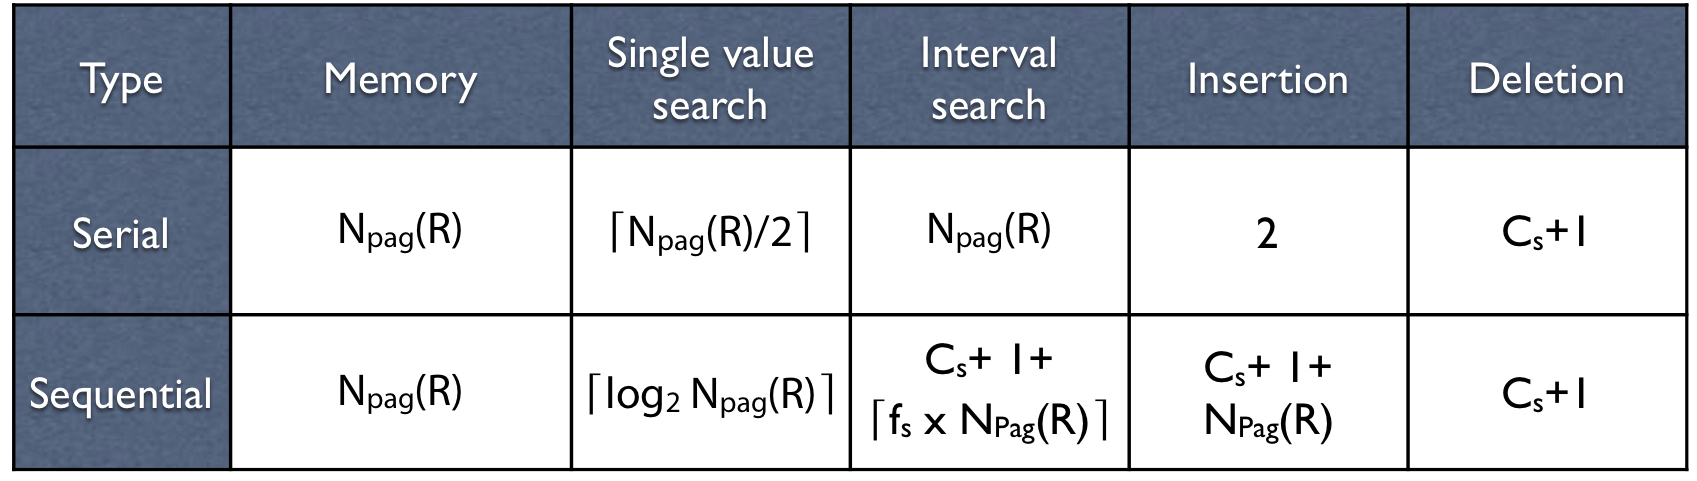
\includegraphics[width=0.7\linewidth]{images/DBMS_Internals/comparison_cost_table.jpeg}
\end{figure}

\begin{itemize}
    \item \textbf{Memory Requirements:} If record insertions are not allowed, the organization requires the same memory as a heap organization.
    \item \textbf{Equality Search}: The cost of a search by a key value both when the value exists in the file and when the value does not exist, is:
    \[\lceil N_{pag}(R) \rceil\]
    If the data is stored in \textit{consecutive pages}, then a binary search has the cost:
    \[\lceil lg N_{pag}(R) \rceil\]
    
    \item \textbf{Range Search}:
    \begin{itemize}
        \item A search by the \textit{key} \(k\) in the range \((k_1 \leq k \leq k_2)\)
        \item Assuming keys numerical uniformly distributed in the range \((k_{min}, k_{max})\)
        \item The \textit{ratio} \(s_f = (k_2 - k_1) / (k_{max} - k_{min})\) called \textbf{selectivity factor} is an estimator of the fraction of pages occupied by the records
        \item And the cost of this operation is:
        \[C_s = \rceil lg N_{pag}(R) \lceil + \rceil s_f \times N_{pag}(R) \lceil - 1\]
    \end{itemize}
    
    \item \textbf{Insert}:
    \begin{itemize}
        \item If the record must be inserted in a page not full
        \[C_s + 1\]
        \item If all the pages are full, the cost is estimated by assuming that the record must be inserted in the \textit{middle of the file}, so we have to move half of pages \(N_{pag(R)}\) thus the total cost is:
        \[C_s + N_{pag}(R) + 1\]
    \end{itemize}
    \item \textbf{Delete and Update}: \(C_s + 1\) if the update does not change the key on which data is sorted.
\end{itemize}

\section{Comparison of Costs}
%TABLE
This table compares costs for heap and sequential organizations in consecutive pages, with \(C_s\) as the search cost of a key value present in the file.
\begin{itemize}
    \item \textbf{Heap organization}
    \begin{itemize}
        \item \textit{Advantage:} good performance for insertion operations
        \item \textit{Disadvantage:} bad performances for range queries and for equality search
    \end{itemize}
    \item \textbf{Sequential organization}
    \begin{itemize}
        \item \textit{Advantage:} good performance for search operations
        \item \textit{Disadvantage:} bad performances for insertion operations
    \end{itemize}
\end{itemize}

\section{External Sorting}
A frequent operation in a database system is sorting a collection of records. Sorting a file is a different process from sorting a table in the temporary memory, because the number of record is usually too large to be completely stored in the memory available. For this reason, the classic algorithms for sorting tables are not applicable to this problem and an external sorting algorithm is used.

Let \(N_{pag}(R)\) be the number of file pages, and \(B\) the buffer pages available, the classical \textit{external sorting algorithm}, called \textbf{merge-sort} consist in two phases:
\begin{itemize}
    \item The \textbf{sort phase:}
    \begin{itemize}
        \item \(B\) file pages are read into the \textit{buffer}, sorted, and written to the disk
        \item This creates \(n = N_{pag}(R) / B\) sorted subset of records called \textit{runs}, numbered from 1 to \(n\) 
    \end{itemize}
    \item The \textbf{merge phase:}
    \begin{itemize}
        \item It consists of \textit{multiple merge passes}
        \item In each, \(Z = B - 1\) runs are merged using the remaining buffer page for output.
        \item At the end the number of runs are \(n = \lceil n / Z \rceil\)
    \end{itemize}
\end{itemize}
The parameter \(Z\) is called the \textbf{merge order} and \(Z + 1\) buffer pages are needed to proceed with a \textbf{Z-Merge}

\begin{figure}[!h]
    \centering
    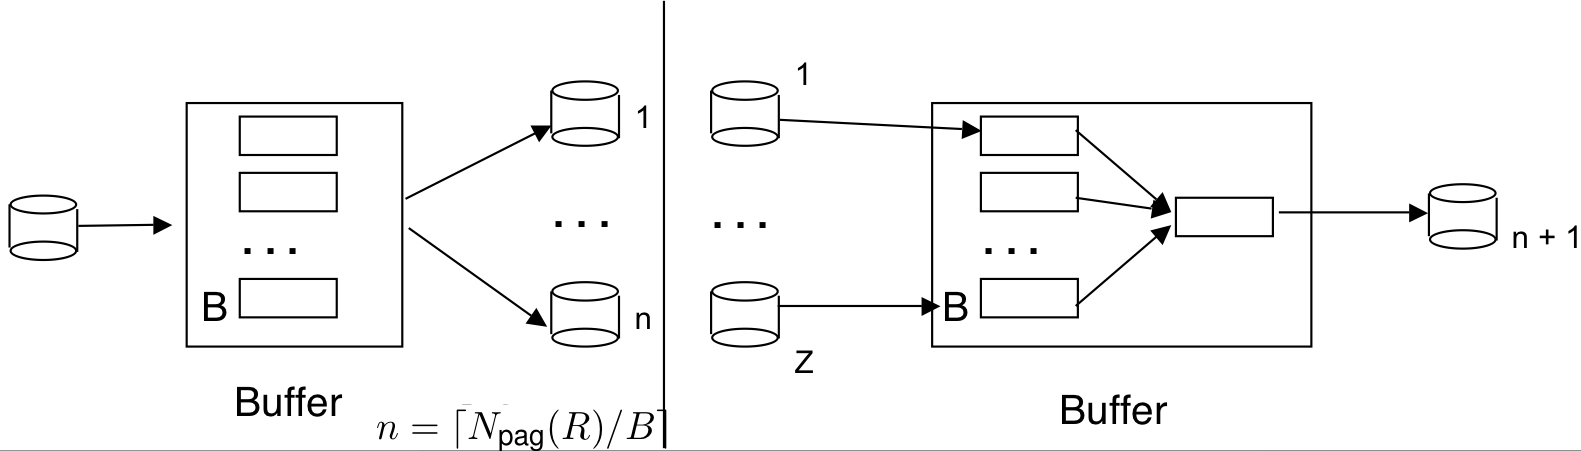
\includegraphics[width=0.7\linewidth]{images/DBMS_Internals/sort_merge.jpeg}
    \caption{Sort-Merge}
\end{figure}


\subsubsection{Example}
Let us show how to sort the file \(A_0\) containing 12 pages, with file and buffer pages capacity of 2 records, \(B = 3\) and 2-merge passes:
\begin{figure}[!h]
    \centering
    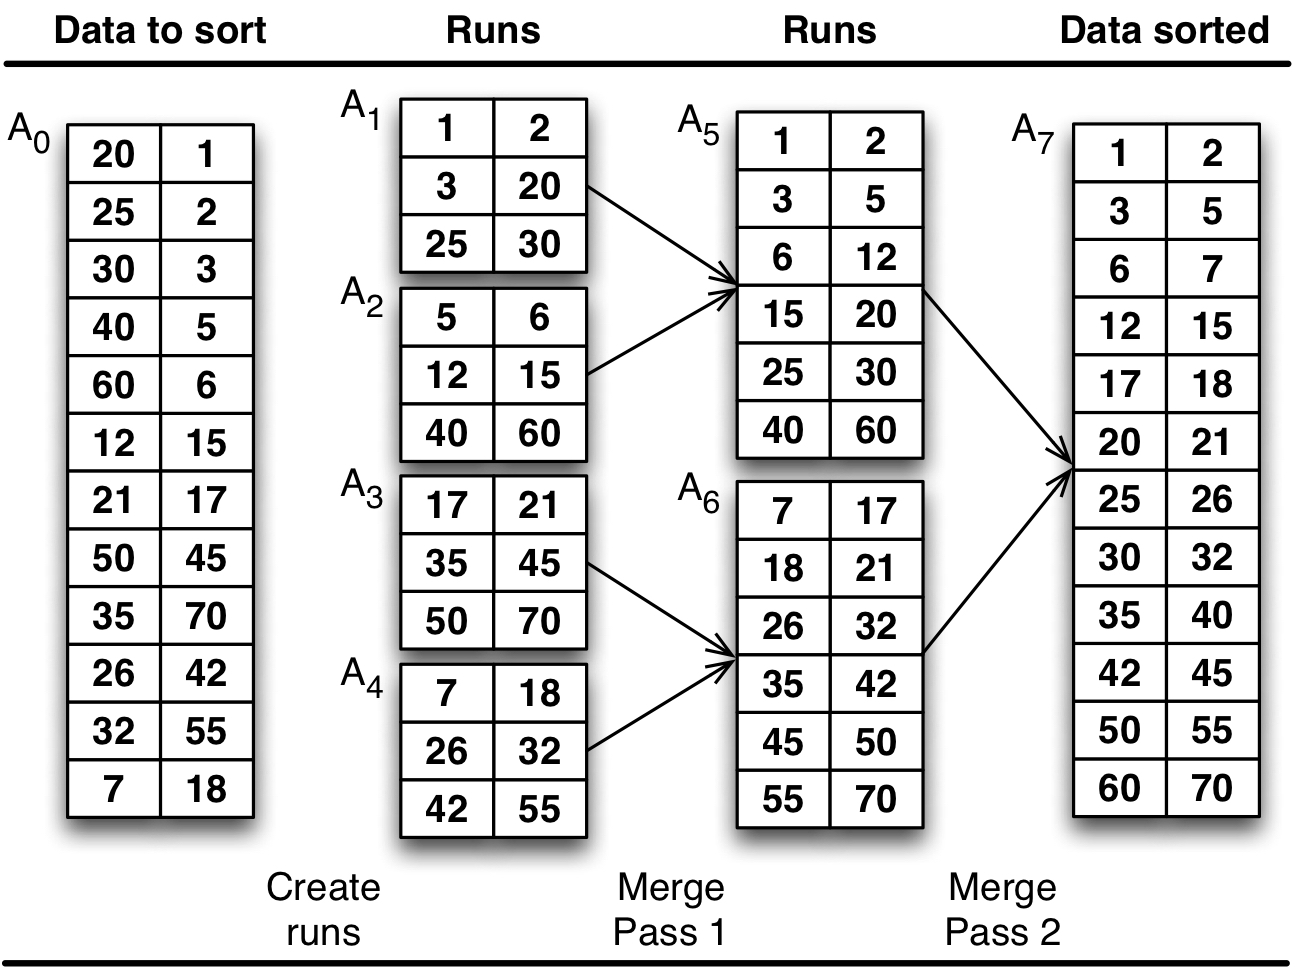
\includegraphics[width=0.7\linewidth]{images/DBMS_Internals/example_sort_merge.jpeg}
    \caption{Example of Sort-Merge}
\end{figure}

\subsection{Performance Evaluation - (NOT REQUIRED)}
\begin{itemize}
    \item Suppose that \(B\) buffer pages are available
    \item The external sorting cost is evaluated in term of number of passes, thus \(N_{pag}(R)\) are read in and written out
    \item The number of passes is the \textit{initial one} to produce the sorted runs, plus the number of the \textit{merge passes}
    \item The \textbf{total cost of the merge-sort algorithm in terms of number of pages:}
    \[C_{sort}(R) = SortPhaseCost + MergePhaseCost\]
    \[C_{sort}(R) = 2 \times N_{pag}(R) + 2 \times N_{pag}(R) \times NoMergePasses\]
    \item If \(N_{pag}(R) \leq B \times (B - 1)\) the data can be sorted with a singe pass, thus the cost becomes:
    \[C_{sort}(R) = 4 \times N_{pag}(R)\]
    \item In general, the number of passes required in the merge phase is a function of the number of file pages \(N_{pag}(R)\), the number \(S\) of initial runs, and the merge order \(Z = B -1\)
    \item After each merge pass, the maximum length of the runs increases of a factor Z, and so their number becomes:
    \[\lceil S/Z \rceil, \lceil S/Z^2 \rceil, \lceil S/Z^3 \rceil...\]
    \item The algorithm terminates when a single run is generated, therefore the number of passes required in the merge phase is:
    \[k = \lceil \log_Z S \rceil\]
    \item Therefore, \textbf{the total cost of the merge-sort is:}
    \[C_{sort}(R) = 2 \times N_{pag}(R) + 2 \times N_{pag}(R) \times \lceil \log_Z S \rceil\]
    \[C_{sort}(R) = 2 \times N_{pag}(R) \times (1 + \lceil \log_Z S \rceil)\]
\end{itemize}